\documentclass[border=10pt]{standalone}
\usepackage{pgfplots}
\pgfplotsset{compat=1.17}
\begin{document}
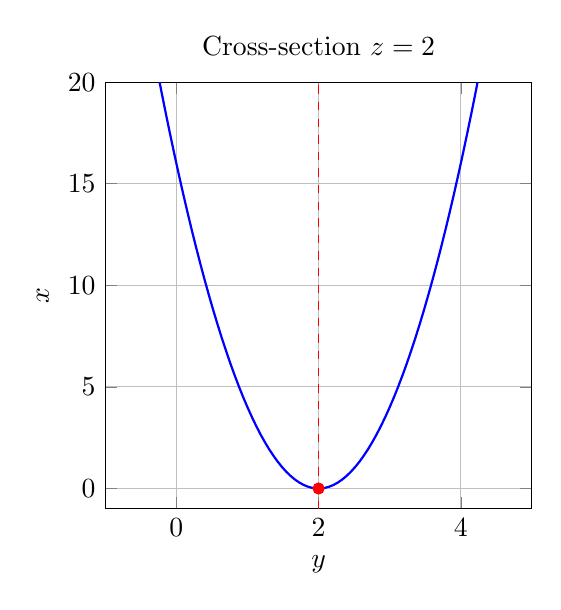
\begin{tikzpicture}
\begin{axis}[
    xlabel={$y$}, ylabel={$x$},
    title={Cross-section $z=2$},
    xmin=-1, xmax=5, ymin=-1, ymax=20,
    grid=both,
    width=7cm, height=7cm,
]
\addplot[blue,thick,domain=-1:5,samples=100] {4*(x-2)^2};
\addplot[red,dashed] coordinates {(2,-1) (2,20)};
\addplot[red,mark=*,mark size=2pt] coordinates {(2,0)};
\end{axis}
\end{tikzpicture}
\hspace{0.5cm}
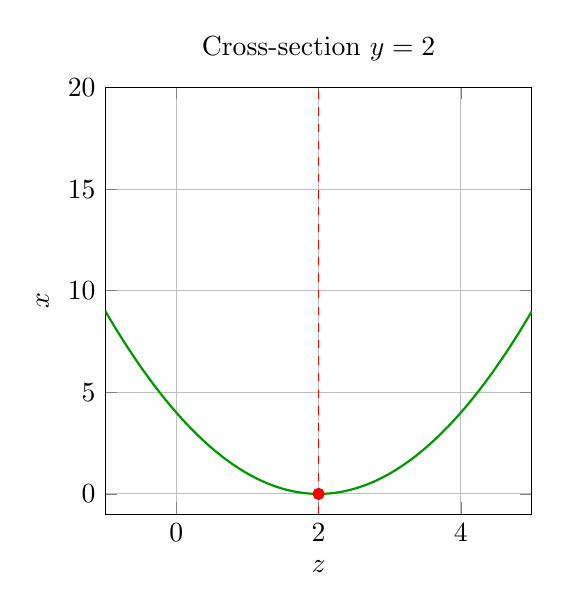
\begin{tikzpicture}
\begin{axis}[
    xlabel={$z$}, ylabel={$x$},
    title={Cross-section $y=2$},
    xmin=-1, xmax=5, ymin=-1, ymax=20,
    grid=both,
    width=7cm, height=7cm,
]
\addplot[green!60!black,thick,domain=-1:5,samples=100] {(x-2)^2};
\addplot[red,dashed] coordinates {(2,-1) (2,20)};
\addplot[red,mark=*,mark size=2pt] coordinates {(2,0)};
\end{axis}
\end{tikzpicture}
\end{document}
